% ======================================================================
% Title: Lecture Notes for MATH1032-01
% Author: Joshua W. Kelly
% Class: MATH1032-01
% Prof. Camren Morgan 
% Date: August 30, 2024
% ======================================================================

\documentclass[12pt]{book}
\usepackage{graphicx}
\usepackage[colorlinks]{hyperref}
\usepackage{amssymb}
\usepackage{amsfonts}
\usepackage{booktabs}
\usepackage{siunitx}
\usepackage{fontawesome}
\usepackage[table]{xcolor}
\usepackage{tikz}
\usepackage{amsmath}
\usepackage[backend=biber]{biblatex}
\addbibresource{calc.bib}
\usepackage[most]{tcolorbox}
\tcbuselibrary{skins,breakable}

% Creates a new tcolorbox environment for definitions, examples, important notes, formulas, and proofs.
\newtcolorbox{definition}[2][]{breakable,sharp corners, skin=enhancedmiddle jigsaw,parbox=false,
boxrule=0mm,leftrule=2mm,boxsep=0mm,arc=0mm,outer arc=0mm,attach title to upper,
after title={.\ }, coltitle=black,colback=gray!10,colframe=black, title={#2},
fonttitle=\bfseries,#1}

\newtcolorbox{example}[2][]{breakable,sharp corners, skin=enhancedmiddle jigsaw,parbox=false,
boxrule=0mm,leftrule=2mm,boxsep=0mm,arc=0mm,outer arc=0mm,attach title to upper,
after title={.\ }, coltitle=blue,colback=blue!10,colframe=blue, title={#2},
fonttitle=\bfseries,#1}

\newtcolorbox{important}[2][]{breakable,sharp corners, skin=enhancedmiddle jigsaw,parbox=false,
boxrule=0mm,leftrule=2mm,boxsep=0mm,arc=0mm,outer arc=0mm,attach title to upper,
after title={.\ }, coltitle=red,colback=red!10,colframe=red, title={#2},
fonttitle=\bfseries,#1}

\newtcolorbox{formula}[2][]{breakable,sharp corners, skin=enhancedmiddle jigsaw,parbox=false,
boxrule=0mm,leftrule=2mm,boxsep=0mm,arc=0mm,outer arc=0mm,attach title to upper,
after title={.\ }, coltitle=purple,colback=purple!10,colframe=purple, title={#2},
fonttitle=\bfseries,#1}

\newtcolorbox{proof}[2][]{breakable,sharp corners, skin=enhancedmiddle jigsaw,parbox=false,
boxrule=0mm,leftrule=2mm,boxsep=0mm,arc=0mm,outer arc=0mm,attach title to upper,
after title={.\ }, coltitle=green,colback=green!10,colframe=green, title={#2},
fonttitle=\bfseries,#1}

\title{MATH1023-01: Lecture Notes} % Title of the document
\author{Joshua W. Kelly} % Author of the document
\date{\today} % Date of the document

% ======================================================================
%
% Notes: 
%
% You can use \label{sec:1} to refer to sections in your document, and then us \ref{sec:1} to refer to the section number.
%
% \begin{definition} and \end{definition} (grey) can be used to define a definition in your document. As well as \begin{example} and \end{example} (blue) for examples, \begin{important} and \end{important} (red) for important notes, \begin{formula} and \end{formula} (maroon) for formulas, and \begin{proof} and \end{proof} (green) for proofs.
% 
% \usepackage[colorlinks]{hyperref} allows you to click on the table of contents and it will take you to the section in the document.
%
% \[ \] is used to create standalone a math equation in the document. and \begin{align*} and \end{align*} is used to create a math equation with multiple lines. \( \) is used to create a math equation in the text.
%
% You can use the code below to create a table in your document.
% 
% \rowcolors{3}{gray!10}{white!50}
% \begin{tabular}{*5l} \toprule
% Header 1 & Header 2 \\ \midrule
% Middle Row &Middle Row \\
% Middle Row & Middle Row \\
% Last Row 1 & Last Row 2 \\ \bottomrule
% \end{tabular}
% 
% ======================================================================

\begin{document}

\maketitle % Creates the title page

\section*{Author's Note} % Section without numbering
These lecture notes are a compilation of material from the course Analytic Geometry and Calculus I (MATH1032) at La Roche University for the Fall 2024 Semester, supplemented with personal notes and reflections on the subject matter. My notes may be accessed at \\ \url{https://github.com/JoshuaWKelly/MATH1032-01-Lecture_Notes/tree/main}. The formatting and style of these notes are inspired by the Feynman Lectures on Physics (\url{https://www.feynmanlectures.caltech.edu/}), and aim to present the concepts of calculus and analytic geometry in an engaging and accessible manner -- similar to how Richard Feynman conveyed complex physics topics.

The content primarily draws from \textit{Calculus Volume 1} by Gilbert Strang et al.\cite{strang_calculus_2016}, a foundational text that provides a thorough introduction to calculus. Problems, examples, and exercises referenced in these notes are sourced directly from this textbook unless otherwise noted. The intention is to provide students with a resource that not only follows the course curriculum but also adds depth and clarity to the material covered in lectures.

I hope these notes serve as a helpful guide for anyone studying calculus and encourage further exploration and understanding of the subject.\\

\noindent{Joshua W. Kelly} \\
\textit{La Roche University} \\ 

\newpage

\vfill

\section*{CC0 1.0 Universal (CC0 1.0) Public Domain Dedication}

\textbf{No Copyright}  
\faCreativeCommons~This work is dedicated to the public domain under the Creative Commons Zero (CC0) license. To the extent possible under law, the author has waived all copyright and related or neighboring rights to this work. 

You can copy, modify, distribute and perform the work, even for commercial purposes, all without asking permission. For more information, see \url{https://creativecommons.org/publicdomain/zero/1.0/}.

\tableofcontents % Creates a table of contents

\newpage

\chapter{Important Formulas} % Chapter 1
\section{Linear Functions}
\subsection{Slope-Intercept Form}
\begin{equation} 
    f(x) = mx + b
\end{equation}

\subsection{Point-Slope Form}
\begin{equation}
    y-y_1 = m(x - x_1)
\end{equation}
\subsection{Standard Form}
\begin{equation}
    ax+by = c,
\end{equation}
\begin{equation}
    a+b \neq 0 
\end{equation}
\subsection{Slope Formula}
\begin{equation}
    m = \frac{y_2 - y_1}{x_2 - x_1}
\end{equation}

\section{Quadratic Functions}
\subsection{Vertex Form}
\begin{equation}
    f(x) = a(x-h)^2 + k
\end{equation}

\subsection{Standard Form}
\begin{equation}
    f(x) = ax^2 + bx + c
\end{equation}

\subsection{Quadratic Formula}
\begin{equation}
	x = \frac{-b \pm \sqrt{b^2 - 4ac}}{2a}
\end{equation}

\section{Exponential Functions}
\subsection{Exponential Growth}
\begin{equation}
    f(x) = ab^x
\end{equation}

\subsection{Exponential Decay}
\begin{equation}
    f(x) = ab^{-x}
\end{equation}

\section{Logarithmic Functions}
\subsection{Common Logarithm}
\begin{equation}
    f(x) = \log_b(x)
\end{equation}

\subsection{Natural Logarithm}
\begin{equation}
    f(x) = \ln(x)
\end{equation}

\section{Trigonometric Functions}
\subsection{Sine Function}
\begin{equation}
    f(x) = \sin(x)
\end{equation}

\subsection{Cosine Function}
\begin{equation}
    f(x) = \cos(x)
\end{equation}

\subsection{Tangent Function}
\begin{equation}
    f(x) = \tan(x)
\end{equation}

\section{Limits}
\subsection{Definition of a Limit}
\begin{equation}
    \lim_{x \to a} f(x) = L
\end{equation}

\subsection{Limit Laws}
\begin{equation}
    \lim_{x \to a} [f(x) + g(x)] = \lim_{x \to a} f(x) + \lim_{x \to a} g(x)
\end{equation}

\begin{equation}
    \lim_{x \to a} [f(x) - g(x)] = \lim_{x \to a} f(x) - \lim_{x \to a} g(x)
\end{equation}

\begin{equation}
    \lim_{x \to a} [cf(x)] = c \lim_{x \to a} f(x)
\end{equation}

\begin{equation}
    \lim_{x \to a} [f(x)g(x)] = \lim_{x \to a} f(x) \lim_{x \to a} g(x)
\end{equation}

\begin{equation}
    \lim_{x \to a} \frac{f(x)}{g(x)} = \frac{\lim_{x \to a} f(x)}{\lim_{x \to a} g(x)}
\end{equation}

\begin{equation}
    \lim_{x \to a} [f(x)]^n = [\lim_{x \to a} f(x)]^n
\end{equation}

\begin{equation}
    \lim_{x \to a} \sqrt[n]{f(x)} = \sqrt[n]{\lim_{x \to a} f(x)}
\end{equation}

\begin{equation}
    \lim_{x \to a} \sqrt[n]{f(x)} = \sqrt[n]{\lim_{x \to a} f(x)}
\end{equation}

\begin{equation}
    \lim_{x \to a} f(x)^{g(x)} = \left[\lim_{x \to a} f(x)\right]^{\lim_{x \to a} g(x)}
\end{equation}

\begin{equation}
    \lim_{x \to a} \frac{1}{f(x)} = \frac{1}{\lim_{x \to a} f(x)}
\end{equation}

\begin{equation}
    \lim_{x \to a} \frac{1}{f(x)} = \frac{1}{\lim_{x \to a} f(x)}
\end{equation}

\begin{equation}
    \lim_{x \to a} \frac{1}{f(x)} = \frac{1}{\lim_{x \to a} f(x)}
\end{equation}

\begin{equation}
    \lim_{x \to a} \frac{1}{f(x)} = \frac{1}{\lim_{x \to a} f(x)}
\end{equation}

\begin{equation}
    \lim_{x \to a} \frac{1}{f(x)} = \frac{1}{\lim_{x \to a} f(x)}
\end{equation}

\chapter{Definitions}
\section{Linear Functions}
One of the most important functions in mathematics is the linear function. A linear function is a function that can be written in the form $f(x) = mx + b$, where $m$ is the slope of the line and $b$ is the $y$-intercept.

\section{Unit Circle}
The unit circle is a circle with a radius of 1. It is centered at the origin of the coordinate plane and is used to define the trigonometric functions.

% Credit for unit circle figure: Supreme Aryal. (2010). Example: Unit circle. \textit{TeXample.net}.  https://texample.net/tikz/examples/unit-circle/ Rights: Licensed under CC BY 2.5 https://creativecommons.org/licenses/by/2.5/ 

\begin{center} 
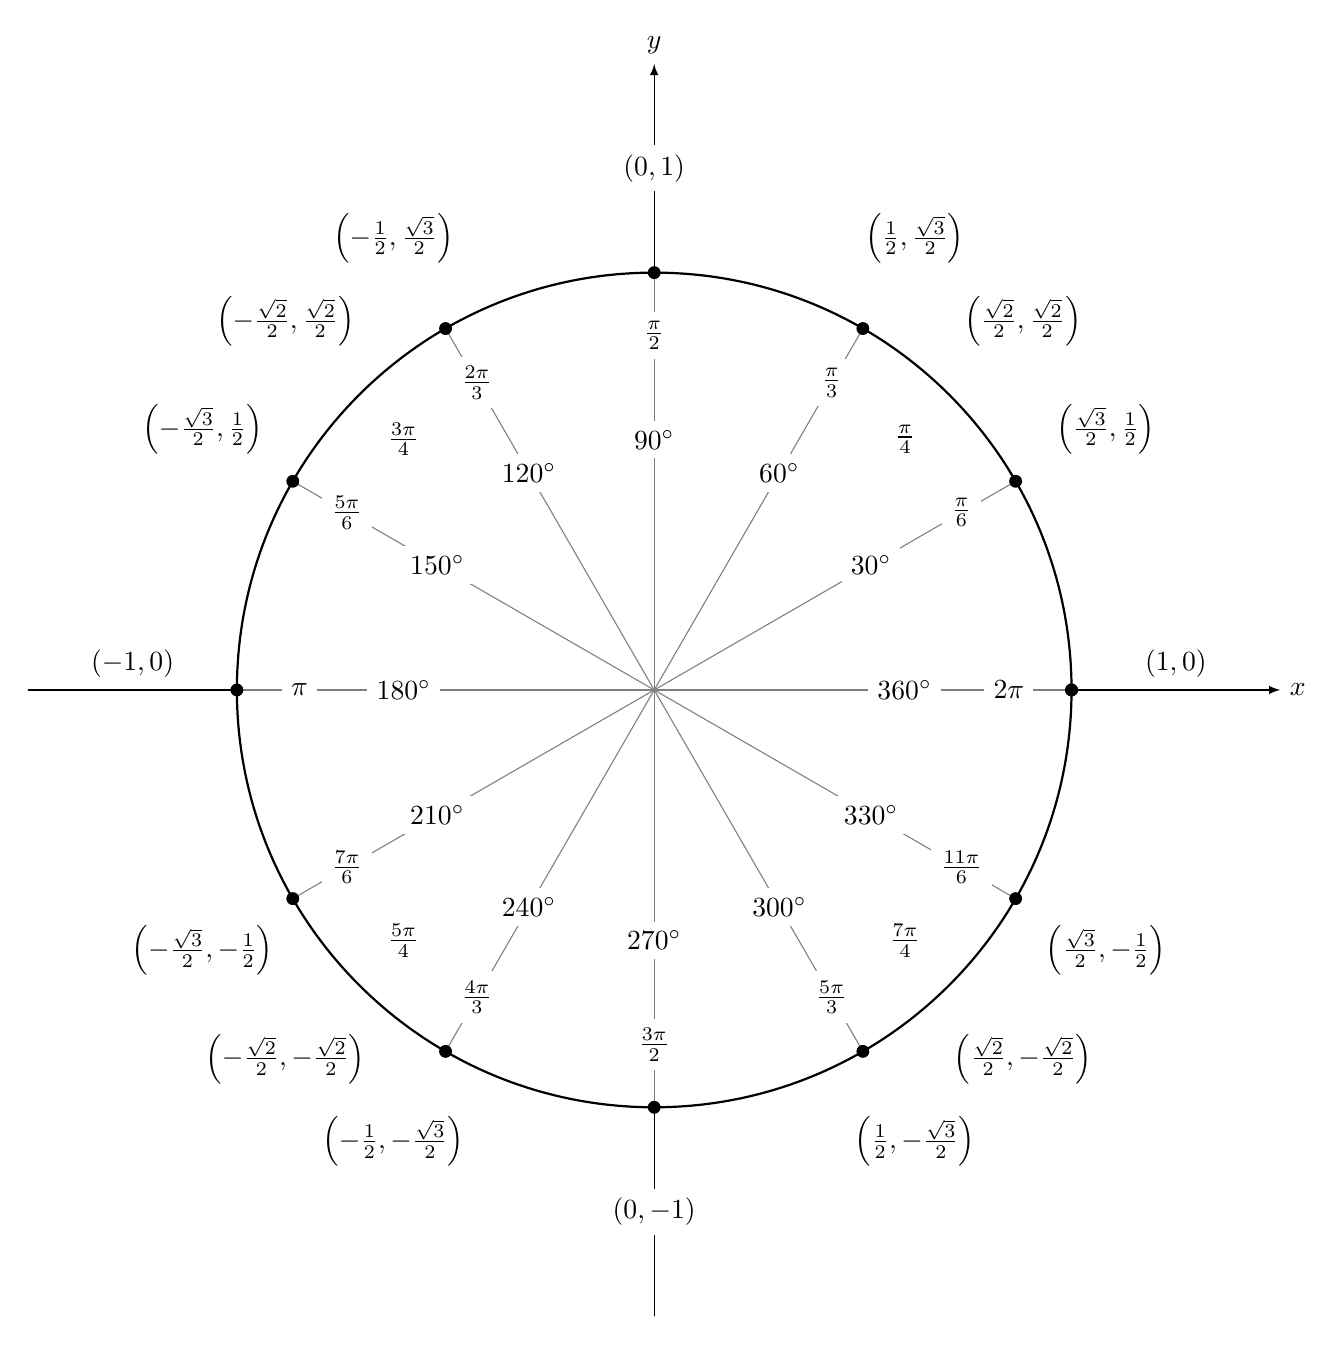
\begin{tikzpicture}[scale=5.3,cap=round,>=latex]
	% draw the coordinates
	\draw[->] (-1.5cm,0cm) -- (1.5cm,0cm) node[right,fill=white] {$x$};
	\draw[->] (0cm,-1.5cm) -- (0cm,1.5cm) node[above,fill=white] {$y$};

	% draw the unit circle
	\draw[thick] (0cm,0cm) circle(1cm);

	\foreach \x in {0,30,...,360} {
			% lines from center to point
			\draw[gray] (0cm,0cm) -- (\x:1cm);
			% dots at each point
			\filldraw[black] (\x:1cm) circle(0.4pt);
			% draw each angle in degrees
			\draw (\x:0.6cm) node[fill=white] {$\x^\circ$};
	}

	% draw each angle in radians
	\foreach \x/\xtext in {
		30/\frac{\pi}{6},
		45/\frac{\pi}{4},
		60/\frac{\pi}{3},
		90/\frac{\pi}{2},
		120/\frac{2\pi}{3},
		135/\frac{3\pi}{4},
		150/\frac{5\pi}{6},
		180/\pi,
		210/\frac{7\pi}{6},
		225/\frac{5\pi}{4},
		240/\frac{4\pi}{3},
		270/\frac{3\pi}{2},
		300/\frac{5\pi}{3},
		315/\frac{7\pi}{4},
		330/\frac{11\pi}{6},
		360/2\pi}
			\draw (\x:0.85cm) node[fill=white] {$\xtext$};

	\foreach \x/\xtext/\y in {
		% the coordinates for the first quadrant
		30/\frac{\sqrt{3}}{2}/\frac{1}{2},
		45/\frac{\sqrt{2}}{2}/\frac{\sqrt{2}}{2},
		60/\frac{1}{2}/\frac{\sqrt{3}}{2},
		% the coordinates for the second quadrant
		150/-\frac{\sqrt{3}}{2}/\frac{1}{2},
		135/-\frac{\sqrt{2}}{2}/\frac{\sqrt{2}}{2},
		120/-\frac{1}{2}/\frac{\sqrt{3}}{2},
		% the coordinates for the third quadrant
		210/-\frac{\sqrt{3}}{2}/-\frac{1}{2},
		225/-\frac{\sqrt{2}}{2}/-\frac{\sqrt{2}}{2},
		240/-\frac{1}{2}/-\frac{\sqrt{3}}{2},
		% the coordinates for the fourth quadrant
		330/\frac{\sqrt{3}}{2}/-\frac{1}{2},
		315/\frac{\sqrt{2}}{2}/-\frac{\sqrt{2}}{2},
		300/\frac{1}{2}/-\frac{\sqrt{3}}{2}}
			\draw (\x:1.25cm) node[fill=white] {$\left(\xtext,\y\right)$};

	% draw the horizontal and vertical coordinates
	% the placement is better this way
	\draw (-1.25cm,0cm) node[above=1pt] {$(-1,0)$}
		  (1.25cm,0cm)  node[above=1pt] {$(1,0)$}
		  (0cm,-1.25cm) node[fill=white] {$(0,-1)$}
		  (0cm,1.25cm)  node[fill=white] {$(0,1)$};
\end{tikzpicture}
\end{center}

Credit: Supreme Aryal \cite{unit} \\ 
Rights: CC BY 2.5

\newpage

\section{Transformations of Functions}

\rowcolors{3}{gray!10}{white!50}
\begin{tabular}{*5l} \toprule
	Transformation of \(f(c>0)\) & Effect on the graph of \(f\) \\ \midrule
   \(f(x)+c\) & Vertical shift up \(c\) units \\
    \(f(x)-c\) & Vertical shift down \(c\) units \\
    \(f(x+c)\) & Shift left by \(c\) units \\
    \(f(x-c)\) & Shift right by \(c\) units \\
	\(cf(x)\) & Vertical Stretch if \(c>1\); vertical compression if \(0<c<1\) \\
	\(f(cx)\) & Horizontal stretch if \(0<c<1\); horizontal compression if \(c>1\) \\
	\(-f(x)\) & Reflection about the \(x\)-axis \\
	\(f(-x)\) & Reflection about the \(y\)-axis \\ \bottomrule
\end{tabular}

	Table 1.7 Transformations of Functions

	\section{Common Angles}

	\rowcolors{3}{gray!10}{white!50}
	\begin{tabular}{*5l} \toprule
		Degrees & Radians & Degrees & Radians \\ \midrule
	   \(0\) & \(0\) & \(120\) & \(\frac{2\pi}{3}\) \\
	\(30\) & \(\frac{\pi}{6}\) & \(135\) & \(\frac{3\pi}{4}\) \\
	\(45\) & \(\frac{\pi}{4}\) & \(150\) & \(\frac{5\pi}{6}\) \\
	\(60\) & \(\frac{\pi}{3}\) & \(180\) & \(\pi\) \\
	\(90\) & \(\frac{\pi}{2}\) & ... & ... \\ \bottomrule
	\end{tabular}

	Table 1.8 Common Angles Expressed in Degrees and Radians

\section{Trigonometric Functions}

	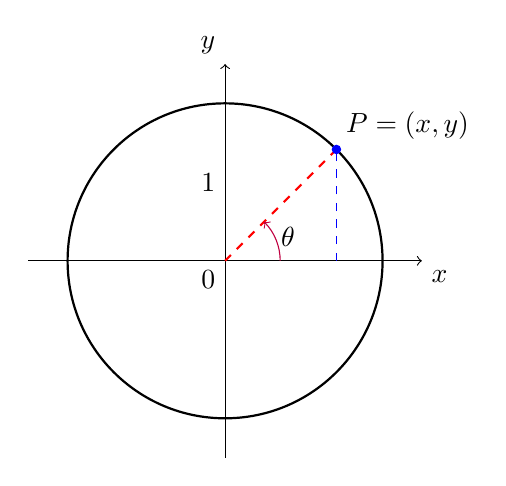
\begin{tikzpicture}
		% Draw the circle
		\draw[thick] (0,0) circle(2cm);
	
		% Draw the x and y axes
		\draw[->] (-2.5, 0) -- (2.5, 0) node[anchor=north west] {$x$};
		\draw[->] (0, -2.5) -- (0, 2.5) node[anchor=south east] {$y$};
	
		% Label 1 on the y-axis
		\node[anchor=east] at (0,1) {$1$};
	
		% Draw the radius line to point P
		\draw[red, thick, dashed] (0,0) -- (45:2);
	
		% Draw the vertical line from x-axis to point P
		\draw[blue, dashed] ({2*cos(45)}, 0) -- ({2*cos(45)}, {2*sin(45)});
	
		% Mark the point P
		\filldraw[blue] (45:2) circle(1.5pt);
		\node[anchor=south west] at (45:2) {$P = (x, y)$};
	
		% Label the origin
		\node[anchor=north east] at (0,0) {$0$};
	
		% Draw the angle theta
		\draw[purple, ->] (0.7,0) arc[start angle=0, end angle=45, radius=0.7cm];
		\node at (0.8, 0.3) {$\theta$};
	
	\end{tikzpicture}

	\textbf{Figure 1.31} The angle \(0\) is in standard position. The values of the trigonometric functions for \(0\) are defined in terms of the coordinates \(x\) and \(y\).

	\newpage 
Let \(P=(x,y)\) be a point on the unit circle centered at the origin \(O\). Let \(\theta\) be an angle with an initial side along the positive \(x\)-axis and a terminal side given by the segment \(OP\). The \textbf{trigonometric functions} are then defined as 

\[\sin\theta=y\]
\[\cos\theta=x\]
\[\tan\theta=\frac{y}{x}\]
\[\csc\theta=\frac{1}{y}\]
\[\sec\theta=\frac{1}{x}\]
\[\cot\theta=\frac{x}{y}\]

If \(x=0\), \(\sec\theta\), and \(\tan\theta\) are defined. If \(y=0\), then \(\cot\theta\) and \(\csc \theta\) are undefined. 

\subsection{Trigonometric Identities} 
\subsubsection{Reciprocal Identities}

\begin{equation}
	\tan \theta = \frac{\sin\theta}{\cos \theta}
\end{equation}

\begin{equation} 
	\csc \theta = \frac{1}{\sin \theta}
\end{equation}

\begin{equation} 
	\cot \theta = \frac{\cos \theta}{\sin \theta}
\end{equation}

\begin{equation} 
	\sec \theta = \frac{1}{\cos \theta}
\end{equation}

\subsubsection{Pythagorean identities}

\begin{equation}
	\sin^2 \theta + \cos^2 \theta = 1
\end{equation}

\begin{equation}
	1 + \tan^2 \theta + 1 = \sec^2 \theta
\end{equation}

\begin{equation}
	1 + \cot^2 \theta = \csc^2 \theta
\end{equation}

\subsubsection{Addition and subtraction formulas}
\begin{equation} 
	\sin(\alpha \pm \beta) = \sin \alpha \cos \beta \pm \cos \alpha \sin \beta
\end{equation}

\begin{equation} 
	\cos(\alpha \pm \beta) = \cos \alpha \cos \beta \mp \sin \alpha \sin \beta
\end{equation}

\subsubsection{Double-angle formulas}
\begin{equation}
	\sin 2\theta = 2 \sin \theta \cos \theta
\end{equation}

\begin{equation} 
	\cos (2\theta) = 2\cos^2 \theta -1 =1-2\sin^2 \theta = \cos ^2 \theta - \sin^2 \theta
\end{equation}



\chapter{Review of Functions}
\section{Introduction}


\section{Linear Functions}
A linear function is a function that can be written in the form $f(x) = mx + b$, where $m$ is the slope of the line and $b$ is the $y$-intercept.

\subsection{Hyperbolic Functions}

Hyperbolic cosine 
\begin{equation}
	\cosh x = \frac{e^x + e^{-x}}{2}
\end{equation}

\chapter{Limits}
\section{Introduction}
This is the introduction section of my document.
\section{Intutive Definition of a Limit}
Imagine you’re standing on the shore, looking out at the ocean. You see a boat far away, and it’s moving towards you. As the boat gets closer, it appears larger and clearer, but if it were to keep coming closer indefinitely, it would eventually reach you, right at your feet. Now, we might say that the boat “approaches” you as it moves closer and closer.

In mathematics, a limit is a way of describing what happens when we look at how something changes as we move closer to a certain point. Think of it as focusing on what happens in the “long run” as we approach a specific point, rather than what happens exactly at that point.

Let’s use an example with numbers: Imagine you have a sequence of numbers that gets closer and closer to 10, like 9, 9.9, 9.99, 9.999, and so on. Even though none of these numbers are exactly 10, we can say that “in the limit,” these numbers are approaching 10. The limit of this sequence is 10 because, as we go further along in the sequence, the numbers get arbitrarily close to 10.

In this sense, a limit is about getting closer and closer to something without necessarily ever reaching it. It’s about the behavior of a function or a sequence as we move toward a certain point or as the input grows indefinitely.

In mathematical terms, if we say the limit of \(f(x)\) as \(x\) approaches \(a\) is \(L\), we mean that we can get \(f(x)\) as close as we want to \(L\) by taking x sufficiently close to \(a\), but not necessarily equal to \(a\).

\section{Preview of Calculus}


\begin{formula}
    {Formula}
	\begin{equation} 
		m_{sec}=\frac{f(x)-f(a)}{x-a}
	\end{equation}
\end{formula}



\section{The Limit of A Function}
\section{The Limit Laws}
\section{Continuity}
\section{The Precise Definition of a Limit}

\begin{formula}
    {Precise Definition of a Limit}
	\begin{equation} 
		\lim_{x \to a} f(x) = L
	\end{equation}
\end{formula}



\begin{definition}
    {Definition of a Limit}
    The limit of a function $f(x)$ as $x$ approaches $a$ is $L$ if for every $\epsilon > 0$ there exists a $\delta > 0$ such that if $0 < |x - a| < \delta$, then $|f(x) - L| < \epsilon$.
\end{definition}

\begin{example}
    {Example 1}
  Enter an example here. 
\end{example}

\begin{important} 
    {Important} It is important that... 
\end{important}

\begin{formula}
    {Formula}
    Enter a formula here.
\end{formula}

\begin{proof}
    {Proof} This is a proof 
\end{proof}

\begin{equation} 
    s(t)= \text{position of the object at time $t$}
\end{equation}

\begin{example} 
{Example 2.2}
\[s(t)=16t^2+64\]
a) \([0.49, 0.50]\) \\
\begin{equation}
    \frac{s(0.5)-s(0.49)}{0.5-0.49}=-15.84
\end{equation}
b) \([0.50, 0.51]\) \\
\begin{equation}
    \frac{s(0.51)-s(0.5)}{0.51-0.5}=16.16u
\end{equation}

\end{example}

\chapter{Derivatives}


% Biblography 

\printbibliography

\newpage

\begin{appendix}
\chapter{Appendix}
	One
	
Let $f(x)$ be a $\mathbb{R}$. Then $f(x)$ is a function of $x$ if for each $x$ in the domain of $f(x)$, there is exactly one value of $f(x)$.

\(\text{Let, \space}f(x)=9+5\text{\space where \space}9\neq 0\)

\end{appendix}

\end{document}